% TU Delft Beamer template
% Author: Maarten Abbink
% Delft University of Technology
% March 2014
% Version 2.0
% Based on original version 1.0 of Carl Schneider
\documentclass{beamer}
\usepackage[english]{babel}
\usepackage{calc}
\usepackage[absolute,overlay]{textpos}
\usepackage{animate}
\usepackage{amssymb,amsmath}
\usepackage{booktabs}
\usepackage{textcomp}
\usepackage{graphicx}
\usepackage{multimedia}
\usepackage{subcaption} 

\mode<presentation>{\usetheme{tud}}

\title[Triogen Turbine Optimization]{Triogen Turbine Optimization}
%\subtitle[Effects of height ratio and rotational]{Effects of height ratio and rotational speed}
\subtitle[Properties SU2 and Coolprop]{Properties SU2 and Coolprop}
\institute[TU Delft]{Delft University of Technology}
\author{Stephan Smit}
\date{\today}

% Insert frame before each subsection (requires 2 latex runs)
\AtBeginSubsection[] {
	\begin{frame}<beamer>\frametitle{\titleSubsec}
		\tableofcontents[currentsection,currentsubsection]  % Generation of the Table of Contents
	\end{frame}
}
% Define the title of each inserted pre-subsection frame
\newcommand*\titleSubsec{Next Subsection}
% Define the title of the "Table of Contents" frame
\newcommand*\titleTOC{Outline}

% define a symbol which can be removed if you don't need it
\newcommand{\field}[1]{\mathbb{#1}}
\newcommand{\Zset}{\field{Z}}

\begin{document}

{
% remove the next line if you don't want a background image
\usebackgroundtemplate{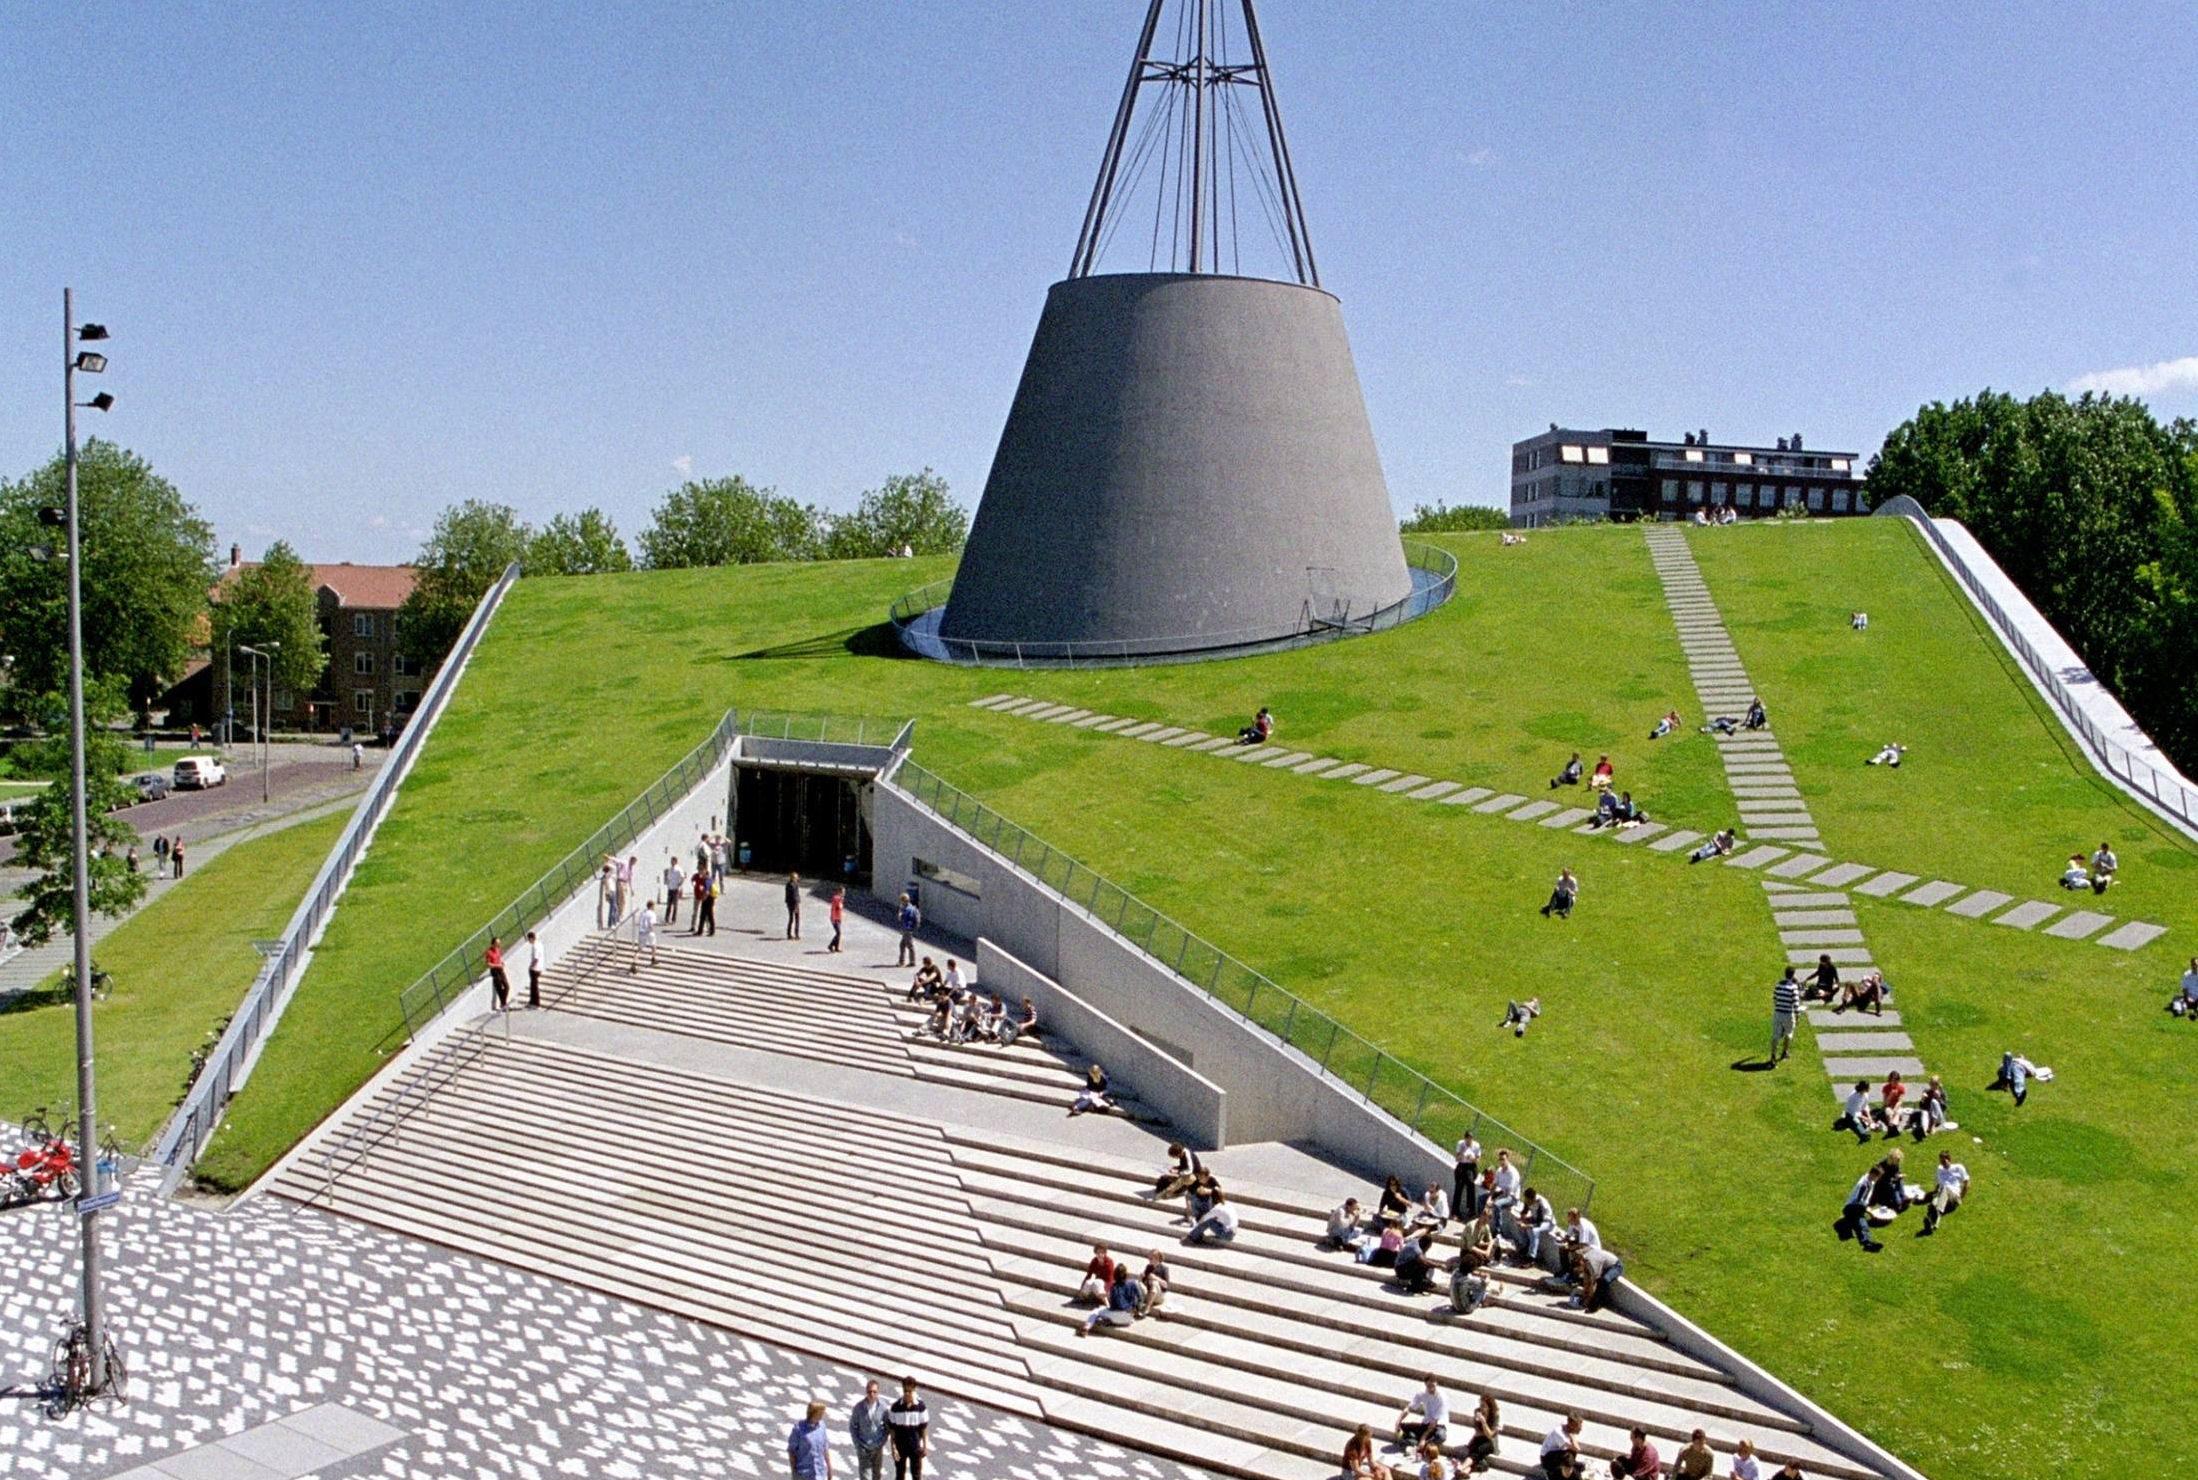
\includegraphics[width=\paperwidth,height=\paperheight]{images/background-titlepage.jpg}}%
\setbeamertemplate{footline}{\usebeamertemplate*{minimal footline}}
\frame{\titlepage}
}


% \section{Fluid Properties}

\section{Variable properties in SU2}

\begin{frame}\frametitle{Variable properties in SU2}
	\begin{itemize}
		\item  Incorporated the visosity model and thermal conductivity model of CoolProp in SU2 
		\begin{itemize}
			\item Reference Correlation of the Viscosity of Toluene from the Triple Point to 675 K and up to 500 MPa (Avgari and Assael, 2015)
			\item Reference Correlation of the Thermal Conductivity of Toluene from the Triple Point to 1000 K and up to 1000 MPa (Assael et al., 2012)
		\end{itemize}
		\item  Peng-Robinson Equation of state used for the thermodynamic properties
		\item  In thermal conductivity model critical correction term not included
		\item  Next figures will show the difference between de CoolProp EOS and the other EOS in SU2
	\end{itemize}
\end{frame}

\begin{frame}\frametitle{Density}
\begin{figure}
\includegraphics[scale=0.6]{../Figures/density.png}
\end{figure}
\end{frame}


\begin{frame}\frametitle{Entropy at constant pressure}
\begin{figure}
\includegraphics[scale=0.6]{../Figures/dsdrho_p.png}
\end{figure}
\end{frame}

\begin{frame}\frametitle{Entropy at constant density}
\begin{figure}
\includegraphics[scale=0.6]{../Figures/dsdp_rho.png}
\end{figure}
\end{frame}


\begin{frame}\frametitle{Enthalpy at constant pressure}
\begin{figure}
\includegraphics[scale=0.6]{../Figures/dhdrho_p.png}
\end{figure}
\end{frame}

\begin{frame}\frametitle{Enthalpy at constant density}
\begin{figure}
\includegraphics[scale=0.6]{../Figures/dhdp_rho.png}
\end{figure}
\end{frame}


\begin{frame}\frametitle{Speed of sound}
\begin{figure}
\includegraphics[scale=0.6]{../Figures/speedofsound.png}
\end{figure}
\end{frame}

\begin{frame}\frametitle{Thermal conductivity}
\begin{figure}
\includegraphics[scale=0.6]{../Figures/thermalconductivity.png}
\end{figure}
\end{frame}

\begin{frame}\frametitle{Viscosity}
\begin{figure}
\includegraphics[scale=0.6]{../Figures/viscosity.png}
\end{figure}
\end{frame}

%{\setbeamertemplate{footline}{\usebeamertemplate*{minimal footline}}
%\begin{frame}\frametitle{\titleTOC}
	%\tableofcontents
%\end{frame}
%}

% \section{Fluid Properties}

% \subsection{Variable properties in SU2}

% \begin{frame}\frametitle{Turbine optimization: Research goals}
% 	\begin{itemize}
% 		\item  Goal: Increase efficiency of Triogen turbine by designing more efficient rotor blade 
% 		\item  One blade every year
% 		\item  After design is manufactured simulations are validated using experiments
% 		% \item  Final design: full 3D adjoint optimization turbinestator and -rotor
% 	\end{itemize}
% \end{frame}
% \begin{frame}

% \begin{frame}
% 	\frametitle{Turbine Geometry}
% 	\begin{figure}
% 	  \begin{subfigure}[b]{0.45\textwidth}
% 	    \includegraphics[width=\textwidth]{images/staggerangles.png}
% 	    \caption{Stagger angles}
% 	    \label{fig:1}
% 	  \end{subfigure}
% 	  \begin{subfigure}[b]{0.45\textwidth}
% 	    \includegraphics[width=\textwidth]{images/leadangles.png}
% 	    \caption{Lead angles}
% 	    \label{fig:2}
% 	  \end{subfigure}
% 	\end{figure}
% \end{frame}



% \begin{frame}
% \frametitle{Effect of Height Ratio}
% \begin{figure}
% \centering    
% \movie[label=show3,width=0.8\textwidth,poster
%        ,autostart=true,showcontrols,loop=true] 
%   {\includegraphics[width=0.6\textwidth]{images/moviestreamlinesHRtemp.png}}{images/moviestreamlineshr.mp4}
%  \end{figure} 
% \end{frame}

% \begin{frame}
% \frametitle{Effect of rotational speed}
% \begin{figure}
% \centering    
% \movie[label=show3,width=0.8\textwidth,poster
%        ,autostart=true,showcontrols,loop=true] 
%   {\includegraphics[width=0.6\textwidth]{images/moviestreamlinesHRtemp.png}}{images/moviemachrot.mp4}
%  \end{figure} 
% \end{frame}

% \begin{frame}
% \frametitle{Effect of rotational speed}
% \begin{figure}
% \centering    
% \movie[label=show3,width=0.8\textwidth,poster
%        ,autostart=true,showcontrols,loop=true] 
%   {\includegraphics[width=0.6\textwidth]{images/moviestreamlinesHRtemp.png}}{images/moviestreamlinesrot.mp4}
%  \end{figure} 
% \end{frame}






% \begin{frame}
% \frametitle{Minimization problem}
	
% 	Design variable vector:
% 	\begin{equation*}
% 	\overline{x}=\begin{bmatrix}
%     x & y & \delta & \beta & \alpha & d
% 	\end{bmatrix}^T
% 	\end{equation*}

% 	Set of all feasible design variables:
% 	\begin{equation*}
% 	  \begin{split}
% 	X =& \{\begin{bmatrix} x & y & \delta & \beta & \alpha \end{bmatrix}^T \in  \mathbb{R}^5: \\ &R<x<R^*,\quad h<y<h^*,\quad  d > 1.0r \}
% 	\end{split}
% 	\end{equation*}
% \end{frame}


% \begin{frame}
% \frametitle{Minimization problem}
% 	Total to static efficiency:
% 	\begin{equation*}
% 	f_{1}(\overline{x})=\eta_{t-s} = \frac{h_{01}-h_{02}}{h_{01}-h_{2s}}
% 	\end{equation*}
% 	Pressure mismatch error:
% 	\begin{equation*}
% 	f_{2}(\overline{x})=\epsilon_p = \frac{\left|P_2-P_{2-desired}\right|}{P_{2-desired}}
% 	\end{equation*}
% 	Minimization problem:
% 	\begin{equation*}
% 	{\begin{aligned}\min &\left(-f_{1}(\overline{x}),f_{2}(\overline{x})\right)\\{\text{s.t. }}&\overline{x}\in X\end{aligned}}
% 	\end{equation*}
% 	Where $X$ is the all set of feasible set of design variables 
% \end{frame}

% \begin{frame}
% \frametitle{Convergence behaviour}
% \begin{figure}
% \includegraphics[scale=0.7]{images/conver.png}
% \end{figure}
% \end{frame}


% \begin{frame}
% \frametitle{Blade}
% \begin{figure}
% \includegraphics[scale=0.7]{images/blade.png}
% \end{figure}
% \end{frame}

% \begin{frame}
% \frametitle{Height}
% \begin{figure}
% \includegraphics[scale=0.7]{images/hd.png}
% \end{figure}
% \end{frame}
% \begin{frame}
% 	\frametitle{Pressure}
% 	\begin{figure}
% 	  \begin{subfigure}[b]{0.45\textwidth}
% 	    \includegraphics[width=\textwidth]{images/InletPressure.png}
% 	    \caption{Inlet Rotor}
% 	    \label{fig:1}
% 	  \end{subfigure}
% 	  \begin{subfigure}[b]{0.45\textwidth}
% 	    \includegraphics[width=\textwidth]{images/OutletPressure.png}
% 	    \caption{Outlet Rotor}
% 	    \label{fig:2}
% 	  \end{subfigure}
% 	\end{figure}
% \end{frame}


% \begin{frame}
% 	\frametitle{Absolute Mach}
% 	\begin{figure}
% 	  \begin{subfigure}[b]{0.45\textwidth}
% 	    \includegraphics[width=\textwidth]{images/InletMach.png}
% 	    \caption{Inlet Rotor}
% 	    \label{fig:1}
% 	  \end{subfigure}
% 	  \begin{subfigure}[b]{0.45\textwidth}
% 	    \includegraphics[width=\textwidth]{images/OutletMach.png}
% 	    \caption{Outlet Rotor}
% 	    \label{fig:2}
% 	  \end{subfigure}
% 	\end{figure}
% \end{frame}


% \begin{frame}
% 	\frametitle{Absolute Radial Mach}
% 	\begin{figure}
% 	  \begin{subfigure}[b]{0.45\textwidth}
% 	    \includegraphics[width=\textwidth]{images/InletRMach.png}
% 	    \caption{Inlet Rotor}
% 	    \label{fig:1}
% 	  \end{subfigure}
% 	  \begin{subfigure}[b]{0.45\textwidth}
% 	    \includegraphics[width=\textwidth]{images/OutletRMach.png}
% 	    \caption{Outlet Rotor}
% 	    \label{fig:2}
% 	  \end{subfigure}
% 	\end{figure}
% \end{frame}

% \begin{frame}
% 	\frametitle{Absolute Tangential Mach}
% 	\begin{figure}
% 	  \begin{subfigure}[b]{0.45\textwidth}
% 	    \includegraphics[width=\textwidth]{images/InletThetaMach.png}
% 	    \caption{Inlet Rotor}
% 	    \label{fig:1}
% 	  \end{subfigure}
% 	  \begin{subfigure}[b]{0.45\textwidth}
% 	    \includegraphics[width=\textwidth]{images/OutletThetaMach.png}
% 	    \caption{Outlet Rotor}
% 	    \label{fig:2}
% 	  \end{subfigure}
% 	\end{figure}
% \end{frame}

% \begin{frame}
% 	\frametitle{Relative Mach}
% 	\begin{figure}
% 	  \begin{subfigure}[b]{0.45\textwidth}
% 	    \includegraphics[width=\textwidth]{images/InletRelMach.png}
% 	    \caption{Inlet Rotor}
% 	    \label{fig:1}
% 	  \end{subfigure}
% 	  \begin{subfigure}[b]{0.45\textwidth}
% 	    \includegraphics[width=\textwidth]{images/OutletRelMach.png}
% 	    \caption{Outlet Rotor}
% 	    \label{fig:2}
% 	  \end{subfigure}
% 	\end{figure}
% \end{frame}








% \begin{frame}
% 	\frametitle{Absolute Flow Angle}
% 	\begin{figure}
% 	  \begin{subfigure}[b]{0.45\textwidth}
% 	    \includegraphics[width=\textwidth]{images/InletFlowAngle.png}
% 	    \caption{Inlet Rotor}
% 	    \label{fig:1}
% 	  \end{subfigure}
% 	  \begin{subfigure}[b]{0.45\textwidth}
% 	    \includegraphics[width=\textwidth]{images/OutletFlowAngle.png}
% 	    \caption{Outlet Rotor}
% 	    \label{fig:2}
% 	  \end{subfigure}
% 	\end{figure}
% \end{frame}


% \begin{frame}
% 	\frametitle{Relative Flow Angle}
% 	\begin{figure}
% 	  \begin{subfigure}[b]{0.45\textwidth}
% 	    \includegraphics[width=\textwidth]{images/InletRelFlowAngle.png}
% 	    \caption{Inlet Rotor}
% 	    \label{fig:1}
% 	  \end{subfigure}
% 	  \begin{subfigure}[b]{0.45\textwidth}
% 	    \includegraphics[width=\textwidth]{images/OutletRelFlowAngle.png}
% 	    \caption{Outlet Rotor}
% 	    \label{fig:2}
% 	  \end{subfigure}
% 	\end{figure}
% \end{frame}


% \begin{frame}
% 	\frametitle{Losses}
% 	\begin{figure}
% 	  \begin{subfigure}[b]{0.45\textwidth}
% 	    \includegraphics[width=\textwidth]{images/pressloss.png}
% 	    \caption{Pressure Losses}
% 	    \label{fig:1}
% 	  \end{subfigure}
% 	  \begin{subfigure}[b]{0.45\textwidth}
% 	    \includegraphics[width=\textwidth]{images/kineticenergyloss.png}
% 	    \caption{Kinetic Energy Losses}
% 	    \label{fig:2}
% 	  \end{subfigure}
% 	\end{figure}
% \end{frame}


% \begin{frame}
% 	\frametitle{Efficiencies}
% 	\begin{figure}
% 	  \begin{subfigure}[b]{0.45\textwidth}
% 	    \includegraphics[width=\textwidth]{images/totaltostatic.png}
% 	    \caption{Total-to-Static}
% 	    \label{fig:1}
% 	  \end{subfigure}
% 	  \begin{subfigure}[b]{0.45\textwidth}
% 	    \includegraphics[width=\textwidth]{images/totaltototal.png}
% 	    \caption{Total-to-Total}
% 	    \label{fig:2}
% 	  \end{subfigure}
% 	\end{figure}
% \end{frame}


% \begin{frame}
% \frametitle{"Original": Absolute Mach}
% \begin{figure}
% \includegraphics[scale=0.052]{images/original/Mach.png}
% \end{figure}
% \end{frame}


% \begin{frame}
% \frametitle{Optimized: Pressure}
% \begin{figure}
% \includegraphics[scale=0.059]{images/optimized/Pressure.png}
% \end{figure}
% \end{frame}


% \begin{frame}
% \frametitle{"Original": Pressure}
% \begin{figure}
% \includegraphics[scale=0.052]{images/original/Pressure.png}
% \end{figure}
% \end{frame}


% \begin{frame}
% \frametitle{Optimized: Velocity}
% \begin{figure}
% \includegraphics[scale=0.059]{images/optimized/Velocity.png}
% \end{figure}
% \end{frame}


% \begin{frame}
% \frametitle{"Original": Velocity}
% \begin{figure}
% \includegraphics[scale=0.052]{images/original/Velocity.png}
% \end{figure}
% \end{frame}

% \begin{frame}
% \frametitle{Optimized: Relative Mach}
% \begin{figure}
% \includegraphics[scale=0.050]{images/optimized/RelMach.png}
% \end{figure}
% \end{frame}

% \begin{frame}
% \frametitle{"Original": Relative Mach}
% \begin{figure}
% \includegraphics[scale=0.059]{images/original/RelMach.png}
% \end{figure}
% \end{frame}


% \begin{frame}
% \frametitle{Optimized: Relative Velocity}
% \begin{figure}
% \includegraphics[scale=0.050]{images/optimized/RelVelocity.png}
% \end{figure}
% \end{frame}

% \begin{frame}
% \frametitle{"Original": Relative Velocity}
% \begin{figure}
% \includegraphics[scale=0.059]{images/original/RelVelocity.png}
% \end{figure}
% \end{frame}



% \begin{frame}
% \begin{table}
% \caption{Characteristic values of best individual:\hspace{\textwidth} $\omega_c=426$ [rpm],$\eta_{t-s}=69.4\%$}
% \begin{tabular}{lrrr}
% \toprule
% {} &    StatorIn &    RotorIn &  RotorOut \\
% \midrule
% Pressure [Pa]              &  3194840.00 &   56323.80 &   9329.13 \\
% Theta-Velocity [m/s]       &       -0.00 &    -527.37 &     -1.96 \\
% Flow-Angle [\textdegree]    &        0.01 &      71.36 &      0.35 \\
% RelFlow-Angle [\textdegree] &        0.01 &      50.89 &    -36.43 \\
% R-Velocity [m/s]           &       -1.79 &    -177.91 &   -278.42 \\
% Temperature [K]            &      587.65 &     448.00 &    416.69 \\
% Energy [J/kg]              & 81603300.00 & 1167170.00 & 166178.00 \\
% Entropy [J/kgK]            &     9128.84 &    9148.74 &   9198.47 \\
% Z-Velocity [m/s]           &        0.00 &       1.10 &      8.13 \\
% Mach [-]                   &        0.01 &       2.72 &      1.45 \\
% Relative Mach [-]          &        0.01 &       1.38 &      1.79 \\
% \bottomrule
% \end{tabular}
% \end{table}

% \end{frame}


% \begin{frame}
% \begin{table}
% \caption{Characteristic values of "original" design:\hspace{\textwidth}$\omega_c=426$ [rpm], $\eta_{t-s}=61.6\%$}
% \begin{tabular}{lrrr}
% \toprule
% {} &    StatorIn &    RotorIn &  RotorOut \\
% \midrule
% Pressure [Pa]              &  3194840.00 &   87313.00 &   6664.92 \\
% Theta-Velocity [m/s]       &       -0.00 &    -509.18 &    -28.88 \\
% Flow-Angle [\textdegree]    &        0.01 &      76.84 &      4.30 \\
% RelFlow-Angle [\textdegree] &        0.01 &      59.40 &    -25.67 \\
% R-Velocity [m/s]           &       -1.79 &    -119.21 &   -381.76 \\
% Temperature [K]            &      587.65 &     459.37 &    402.10 \\
% Energy [J/kg]              & 81603300.00 & 1770970.00 & 124977.00 \\
% Entropy [J/kgK]            &     9128.84 &    9148.61 &   9172.80 \\
% Z-Velocity [m/s]           &        0.00 &       0.32 &     52.34 \\
% Mach [-]                   &        0.01 &       2.54 &      1.99 \\
% Relative Mach [-]          &        0.01 &       1.14 &      2.20 \\
% \bottomrule
% \end{tabular}
% \end{table}
% \end{frame}



% \begin{frame}
% \frametitle{Preliminary conclusions}
% 	\begin{itemize}
% 		\item Original and optimized are not directly comparable as the outlet conditions are not the same 
% 		\item The height of the blade has more than doubled, this needs to be accounted for in blade thickness to ensure structural integrity
% 		\item Optimizations take a lot longer due to busy cluster, this slows down the iterative improvement of the optimization and testing of different hypotheses
% 	\end{itemize}
% \end{frame}


% \begin{frame}
% \frametitle{What am I doing now}
% 	\begin{itemize}
% 		\item Running optimization with different constraint on thickness 
% 		\item Started developing Surrogate Model to reduce computational time
% 			\begin{itemize}
% 				\item an out-of-the box Kriging model has been developed but needs to be included in the optimization routine
% 			\end{itemize}
% 		\item Started cooperation with master-student of Nitish $\rightarrow$ will lead to incorporating the MOC-code of Nitish in the optimization code
% 	\end{itemize}
% \end{frame}


% \begin{frame}
% \frametitle{Discussion}
% 	\begin{itemize}
% 		\item How to turn these optimization results into a quick and dirty design?
% 			\begin{itemize}
% 				\item Possible idea: take found angles and camberline, and height distribution, assume rule of thumb thickness and generate new design
% 			\end{itemize}
% 		\item Optimizer tried to make the blade as thin as possible, what is a reasonable constraint for this, also taking into account the increase height?
% 	\end{itemize}
% \end{frame}

% \begin{frame}
% \frametitle{Relative Velocity}
% \begin{figure}
% \includegraphics[scale=0.05]{images/RelVelocity2.png}
% \end{figure}
% \end{frame}

% \begin{frame}
% \frametitle{Extended mesh}
% \begin{figure}
% \includegraphics[scale=0.05]{images/mesh-side.png}
% \end{figure}
% \end{frame}

% \begin{frame}
% \frametitle{Inviscid simulation: Absolute velocity}
% \begin{figure}
% \includegraphics[scale=0.05]{images/Velocity.png}
% \end{figure}
% \end{frame}

% \begin{frame}
% \frametitle{Inviscid simulation: Absolute velocity}
% \begin{figure}
% \includegraphics[scale=0.05]{images/Velocity-zoom.png}
% \end{figure}
% \end{frame}

% \begin{frame}
% \frametitle{Inviscid simulation: Absolute velocity }
% \begin{figure}
% \includegraphics[scale=0.05]{images/Velocity-top.png}
% \end{figure}
% \end{frame}

% \begin{frame}
% \frametitle{Inviscid simulation: Relative velocity }
% \begin{figure}
% \includegraphics[scale=0.05]{images/RelVelocity-zoom.png}
% \end{figure}
% \end{frame}
% \begin{frame}

% \frametitle{Inviscid simulation: Relative velocity }
% \begin{figure}
% \includegraphics[scale=0.05]{images/RelVelocity-side.png}
% \end{figure}
% \end{frame}

% \begin{frame}
% \frametitle{Inviscid simulation: Static pressure }
% \begin{figure}
% \includegraphics[scale=0.05]{images/pressure.png}
% \end{figure}
% \end{frame}


% \begin{frame}
% \frametitle{Inviscid simulation: Temperature }
% \begin{figure}
% \includegraphics[scale=0.05]{images/Temperature.png}
% \end{figure}
% \end{frame}

% \begin{frame}
% \frametitle{Viscous optimizations: characteristic values}
% \begin{table}[]
% 	\centering
% 	\caption{Simulation results: rotational speed 426 Hz}
% 	\label{my-label}
% 		\begin{tabular}{|l|l|l|}
% 		\cline{1-3}
% 			                          & Optimization 1 & Optimization 2 &\\ \cline{1-3}
% 		Total-static efficiency       &    1.82     &   1.7      	\\ \cline{1-3}
% 		Pressure {[}Bar{]}            &       31.98      &  1      &  \\ \cline{1-3}
% 		Mach  {}      				  &       0.01       &     2.4467        &  \\ \cline{1-3}
% 		Abs. Flow angle {[}deg{]}     &       1.16       &   1       &  \\ \cline{1-3}
% 		Rel. Flow angle {[}deg{]}     &       1.1       &    1 &  \\ \cline{1-3}
% 		\end{tabular}
% 	\end{table}
% \end{frame}


% \begin{frame}
% \frametitle{Possible explanation: Recirculation zone}
% 	\begin{itemize}
% 		\item  Flow after blade passage has still large amount of tangential velocity component
% 		\item  Centrifugal force pushes the flow outwards creating a low pressure zone in the center
% 		\item  Due to pressure gradient between the center and the outflow, mass will flow inwards from the outflow
% 	\end{itemize}
% \end{frame}



% \begin{frame}
% \frametitle{Problems with this simulation}
% 	\begin{itemize}
% 		\item  Flow conditions are not well-defined for this backflow problem
% 		\begin{itemize}
% 			\item massflow out is not equal to mass flow coming in
% 			\item properties are not defined for the backflow coming into the domain
% 		\end{itemize}
% 		\item Possible solutions?
% 		\begin{itemize}
% 			\item Cut of the mesh sooner to avoid recirculation zone
% 			\item But far enough from the blade such that pressure can be matched
% 		\end{itemize}
% 	\end{itemize}
% \end{frame}


% \begin{frame}
% \frametitle{ What needs to be done}
% 	\begin{itemize}
% 		\item Parameterization of Shroud?
% 		\item Conversion from Hub/Shroud to Meridinial line with Area distribution
% 		\begin{itemize}
% 			\item Finding meridinial line not straightforward
% 			\item For the moment we use a camberline-like procedure
% 			\item Function to translate area distribution along the meridinial line to scaled hub and shroud need to be written
% 		\end{itemize}
% 		\item Possible reformulation of optimization cost-function: minimizing swirl?
% 	\end{itemize}
% \end{frame}







% % \begin{frame}
% % \frametitle{Possible alternative plan?}
% % 	\begin{itemize}
% % 		\item  Take current bladeshape and keep this constant
% % 		\item  Only vary the height distribution 
% % 		\item  Extend the mesh of Enrico with a rotated section
% % 		\item  Advantages: 
% % 			\begin{itemize}
% % 				\item First (partly) optimized result can be produced within 2 weeks!
% % 				\item No grid-convergence study neccesary (sufficiently fine grid [for blade region] already avaible by Enrico)
% % 			\end{itemize}	
% % 		\item Required items to do:
% % 		\begin{itemize}
% % 			\item script to read in mesh, change height,name boundaries, add rotated section, export ($\sim$ 2 days)
% % 			\item turn on multi-objective optimization and wait ($\sim$ 3 days)
% % 			\item incorporate new height distribution in CAD geometry (? days)
% % 		\end{itemize}	
% % 	\end{itemize}
% % \end{frame}




% %\subsection{Section 2 - Subsection 1}

% %\begin{frame}\frametitle{Data-driven RANS modeling: Adjoint method}
% %\begin{multline*}
% %	R(\theta, \beta) = \frac{\partial}{\partial y} \left(\alpha\frac{\partial \theta }{\partial y } + \beta \right) + Q_r  \\
% %    =\frac{\partial \alpha}{\partial y} \frac{\partial \theta }{\partial y } +\alpha \frac{\partial  ^2\theta}{\partial y ^2}+ \frac{\partial \beta }{\partial y } + Q_r(\theta) = A\theta -b= 0
% %\end{multline*}
% %Where $A=\frac{\partial \alpha}{\partial y} \frac{\partial }{\partial y } +\alpha \frac{\partial  ^2}{\partial y ^2}$ and $b = -Q_r - \frac{\partial \beta}{\partial y}$
% %\end{frame}

% %\begin{frame}\frametitle{Section 2 - subsection 1 - page 1}
% %	\begin{alertblock}{Alertblock}
% %		This page gives an example with numbered bullets (enumerate)\\
% %		in an "Example" window:\\
% %	\end{alertblock}
	
% %	\begin{example}
% %		Discrete domain $\Rightarrow$ evaluate in each point\\
% %		Not possible for\\
% %		\begin{enumerate}
% %			\item <1-> parametric domains
% %			\item <2-> large domains (NP-complete)
% %		\end{enumerate}
% %	\end{example}
% %\end{frame}

% %\subsection[]{Section 2 - Last Subsection}

% %\begin{frame}\frametitle{Last Page}
% %	\begin{block}{Summary}
% %		\centering{End of the beamer demo\\
% %		with a \emph{tidy} TU~Delft lay-out.\\
% %		Thank you!}
% %	\end{block}
% %\end{frame}

\end{document}
